\documentclass{article}

\usepackage{amsmath, amssymb}
\usepackage{graphicx}


\author{Sebastian Valencia}
\title{Otro ejemplo de \LaTeX}

\begin{document}
\maketitle

\begin{abstract}
Este es otro ejemplo del uso basico de \LaTeX

\end{abstract}

\section{Ecuaciones}
Las ecuaciones en linea, van entre signos de pesos: $F = ma$.\\
Tambien se pueden poner en un entorno propio de ecuaciones:
\begin{equation}
\int y\, \mathrm{d}x
\end{equation}

\begin{equation*}
\left(\!
	\begin{array}
		{c}
      	n \\
      	r
    \end{array}
\!\right) = \frac{n!}{r!(n-r)!}
\end{equation*}

\section{Tablas}
Las tablas en \LaTeX, tienen un entorno especial. \\
Existe un entorno tabular que permite referenciar la tabla \ref{Ta: Notas}. \\

\begin{table}[h] % Para poner en el lugar de definicion
\centering
	\begin{tabular}{| l | c | c | c}
		\hline
		Nombre & Primero & Secundo \\ \hline
		Ana & 5.0 & 3.4 \\ \hline
		Beatriz & 4.2 & 2.4 \\ \hline
		Carlos & 3.4 & 5.0 \\ \hline
	\end{tabular}
\caption{Notas de los parciales}
\label{Ta: Notas}
\end{table}

\pagebreak

\section{Figuras}

\begin{figure}[h]
\centering
	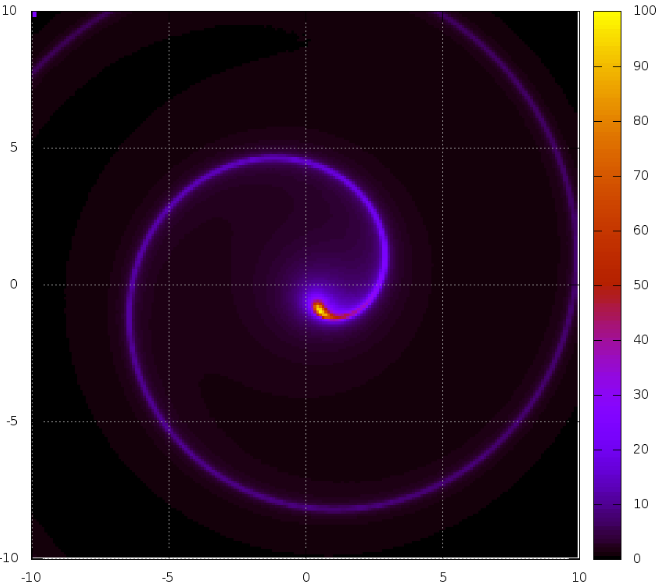
\includegraphics[scale=0.5]{Circulo09c.png}
	\caption{Imagen a 0.9c}
	\label{Fi: Galaxia}
\end{figure}

\end{document}